\capitulo{5}{Aspectos relevantes del desarrollo del proyecto}

\section{Aspectos relevantes del desarrollo del proyecto}

\section{Planificación del proyecto}
La planificación del proyecto se llevó a cabo utilizando un diagrama de Gantt, que permitió una gestión detallada y estructurada de todas las fases del proyecto. Este diagrama se actualizó regularmente para reflejar el progreso y realizar ajustes según las necesidades. La planificación detallada ayudó a asegurar que todas las tareas fueran completadas a tiempo y dentro del alcance definido.

\begin{figure}[H]
	\centering
	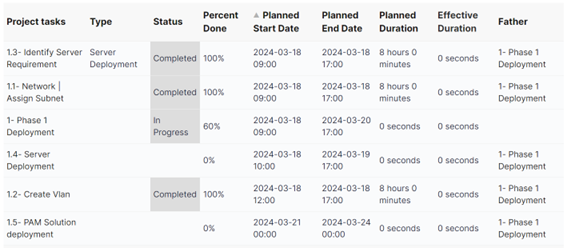
\includegraphics[width=0.8\textwidth]{./img/diagrama1.png}
	\caption{Diagrama del proyecto.}
	\label{fig:diagrama1}
\end{figure}
A continuación, se muestran varias capturas detalladas del diagrama de Gantt, destacando las diferentes fases del proyecto:

\begin{figure}[H]
	\centering
	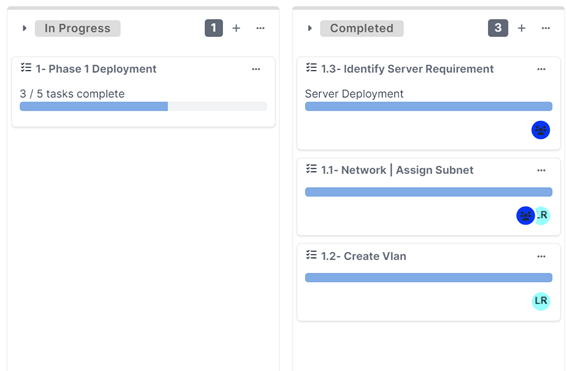
\includegraphics[width=0.8\textwidth]{./img/diagrama2.png}
	\caption{Detalle del diagrama de Gantt.}
	\label{fig:diagrama_detalle1}
\end{figure}

\begin{figure}[H]
	\centering
	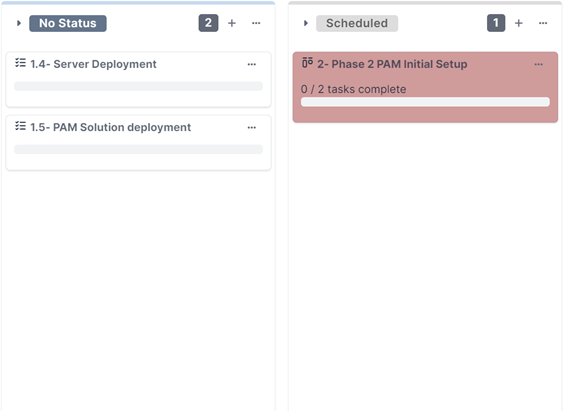
\includegraphics[width=0.8\textwidth]{./img/diagrama3.png}
	\caption{Detalle del diagrama de Gantt: fase de desarrollo.}
	\label{fig:diagrama_detalle2}
\end{figure}


\section{Despliegue de la máquina virtual}
El primer paso del proyecto fue la configuración y despliegue de una máquina virtual en vSphere~\cite{vsphere}. Esta máquina se ha creado con especificaciones adecuadas para soportar PAM360, incluyendo 16 GB de RAM y un sistema operativo Windows Server 2019.

\begin{figure}[H]
	\centering
	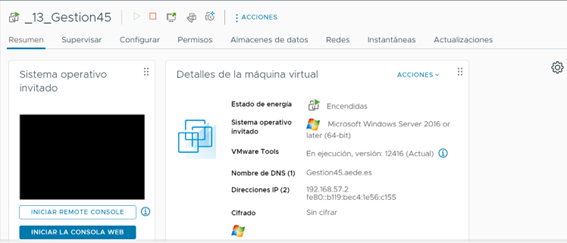
\includegraphics[width=0.8\textwidth]{./img/maquina_pam_vshpere.png}
	\caption{Detalles de la máquina virtual en vSphere.}
	\label{fig:maquina_pam_vshpere}
\end{figure}

\begin{figure}[H]
	\centering
	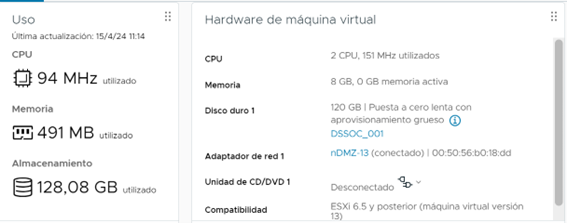
\includegraphics[width=0.8\textwidth]{./img/maquina_pam_detalle.png}
	\caption{Configuración  más detallada de la máquina virtual en vSphere.}
	\label{fig:maquina_pam_vshpere_detalle1}
\end{figure}

\section{Instalación de PAM360}
La instalación de PAM360 se realizó en la máquina virtual utilizando MRemote para la transferencia de archivos y acceso remoto. El proceso de instalación involucró varios pasos, desde la transferencia del archivo ejecutable hasta la configuración inicial del software.

\begin{figure}[H]
	\centering
	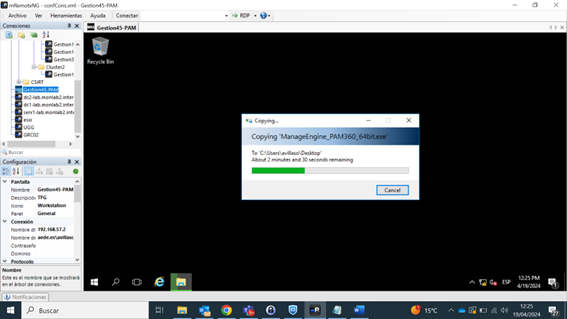
\includegraphics[width=0.8\textwidth]{./img/instalacion_pam.png}
	\caption{Proceso de instalación de PAM360.}
	\label{fig:instalacion_pam}
\end{figure}

\subsection{Proceso de instalación}
El proceso de instalación de PAM360 fue documentado con varias capturas para asegurar la correcta instalación y configuración inicial del software.

\begin{figure}[H]
	\centering
	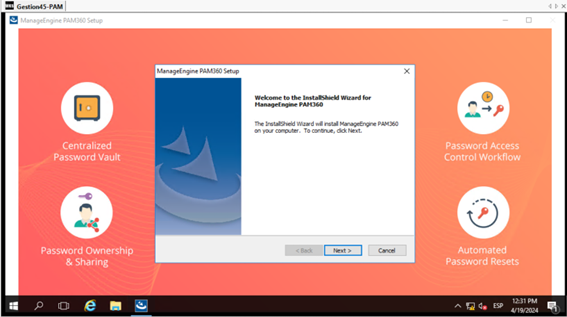
\includegraphics[width=0.8\textwidth]{./img/instalacion_pam2.png}
	\caption{Proceso de instalación de PAM360, primera página.}
	\label{fig:instalacion_detalle1}
\end{figure}

\begin{figure}[H]
	\centering
	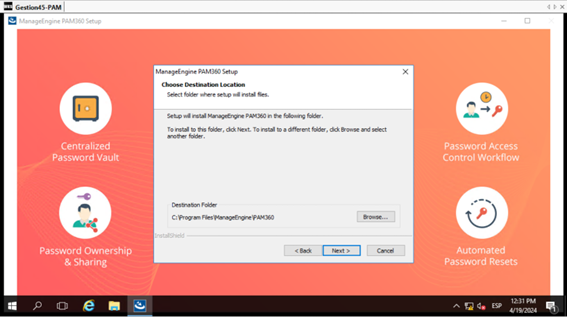
\includegraphics[width=0.8\textwidth]{./img/instalacion_pam3.png}
	\caption{Proceso de instalación de PAM360, segunda página.}
	\label{fig:instalacion_detalle2}
\end{figure}

\begin{figure}[H]
	\centering
	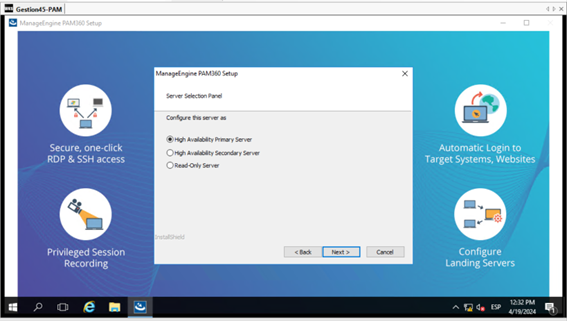
\includegraphics[width=0.8\textwidth]{./img/instalacion_pam4.png}
	\caption{Proceso de instalación de PAM360, tercera y última página.}
	\label{fig:instalacion_detalle3}
\end{figure}

\section{Configuración inicial de PAM360}
Una vez instalado PAM360, se procedió a la configuración inicial, que incluyó el cambio de la contraseña del administrador y la configuración de la autenticación y recursos. Esta fase fue crucial para asegurar que PAM360 estuviera configurado de acuerdo con los requisitos de seguridad de NTT Data.

En las siguientes imágenes se puede observar la aplicación funcionando. 
\begin{figure}[H]
	\centering
	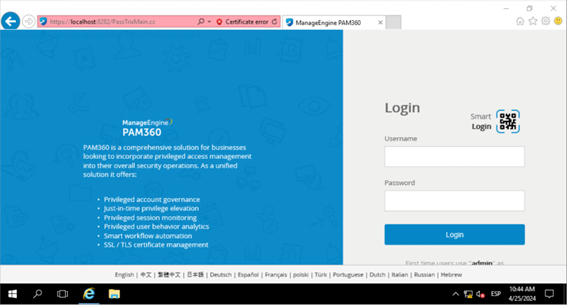
\includegraphics[width=0.8\textwidth]{./img/login_pam_limpio.png}
	\caption{Pantalla principal de PAM.}
	\label{fig:pam_accesoinicial}
\end{figure}


El primer acceso tiene las credenciales por defecto ''admin/admin'' . PAM nos fuerza a que nada más se acceda, se debe cambiar la contraseña por una nueva

\begin{figure}[H]
	\centering
	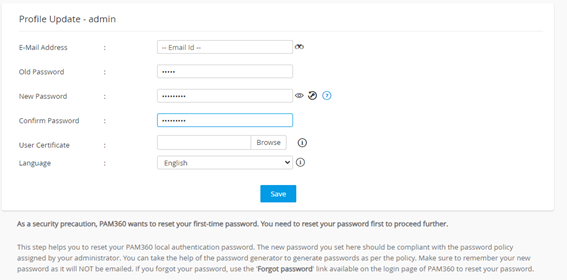
\includegraphics[width=0.8\textwidth]{./img/pam_upadteadmin_pass.png}
	\caption{Configuración del administrador en PAM360.}
	\label{fig:pam_upadteadmin_pass}
\end{figure}

Una vez cambiada, PAM se conectará automáticamente haciéndonos saber que todo ha sido correcto.
\begin{figure}[H]
	\centering
	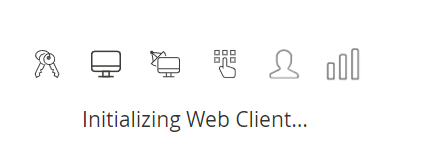
\includegraphics[width=0.8\textwidth]{./img/iniciar_pam.png}
	\caption{Configuración del administrador en PAM360.}
	\label{fig:pam_inicio}
\end{figure}

Dado que no hay ninguna máquina, contraseña o usuario vinculados a la solución, la página podría presentarse de la siguiente manera:

\begin{figure}[H]
	\centering
	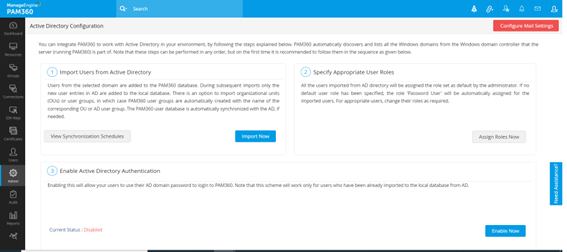
\includegraphics[width=0.8\textwidth]{./img/pam_portada_vanilla.png}
	\caption{Configuración del administrador en PAM360.}
	\label{fig:pam_inicio_limpio}
\end{figure}


\section{Integración con Active Directory}
La integración con Active Directory (AD) fue una de las tareas más importantes del proyecto. Este proceso permitió la importación de usuarios y grupos del AD a PAM360, facilitando el control de acceso y la gestión de credenciales. Se configuró el dominio AD ''NTTDATA'' y se importaron los usuarios necesarios.

\begin{figure}[H]
	\centering
	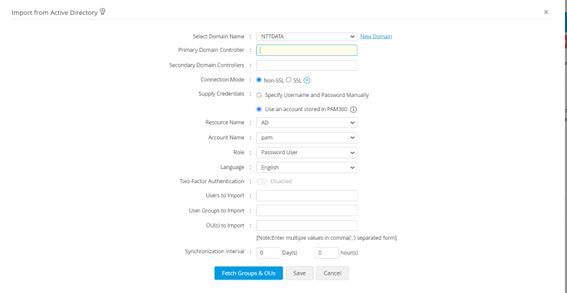
\includegraphics[width=0.8\textwidth]{./img/pam_ad3.png}
	\caption{Importación de usuarios desde Active Directory.}
	\label{fig:pam_ad3}
\end{figure}

Debemos crear una política de password para poder añadir el AD, esto es un requisito adicional de PAM como capa extra de seguridad, para cerciorarse que las contraseñas que pongamos cumplan los requisitos estándar de seguridad.

\begin{figure}[H]
	\centering
	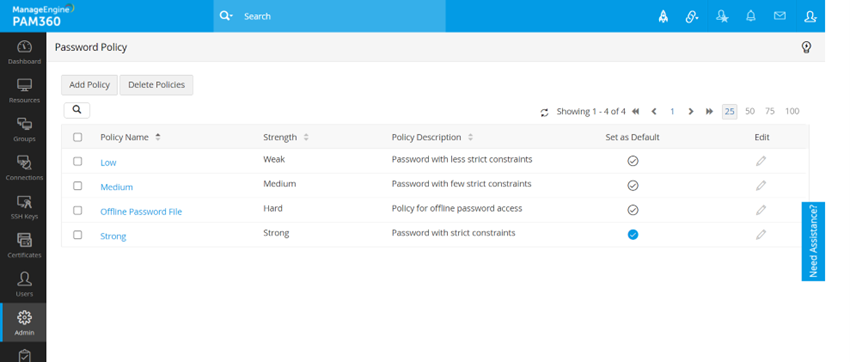
\includegraphics[width=0.8\textwidth]{./img/pam_password_policy.png}
	\caption{Configuración del administrador en PAM360.}
	\label{fig:pam_password_policy}
\end{figure}

Cuando se haya integrado correctamente todo, se debería ver así:

\begin{figure}[H]
	\centering
	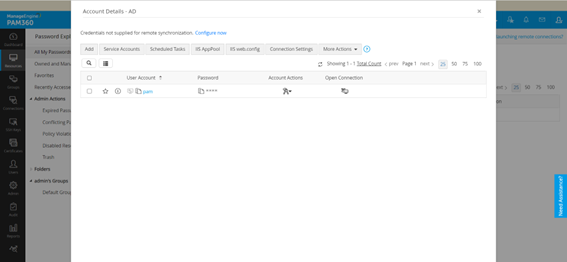
\includegraphics[width=0.8\textwidth]{./img/pam_integradoya_ad.png}
	\caption{AD con la cuenta de pam activo.}
	\label{fig:pam_ad4}
\end{figure}

Una vez creada la entrada para el AD, el siguiente paso era importar los usuarios del AD a los que se vayan a querer dar acceso a las herramientas y así comprobar que la integración con el AD ha sido exitosa.

\begin{figure}[H]
	\centering
	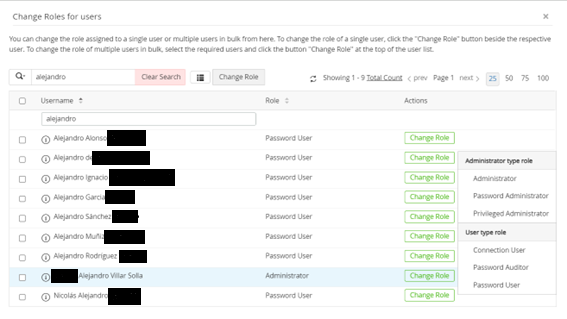
\includegraphics[width=0.8\textwidth]{./img/importacion_usuarios_ad.png}
	\caption{AD con la cuenta de pam activo.}
	\label{fig:pam_ad5}
\end{figure}

Se han censurado los nombres por privacidad de la empresa. Podemos así comprobar que todos los usuarios existentes del AD se han podido traer y vincular correctamente.

\section{Importación de máquinas de nuestro entorno}
Cuando tengamos acceso al AD, podremos importar las máquinas que queramos dar acceso a usuarios. En este caso se han importado ''Gestión41'' y ''Gestion42''. La se realiza de forma similar, seleccionas el nombre, la IP y el SO que se ejecuta en la máquina y PAM automáticamente configura todo lo necesario para el acceso.

\begin{figure}[H]
	\centering
	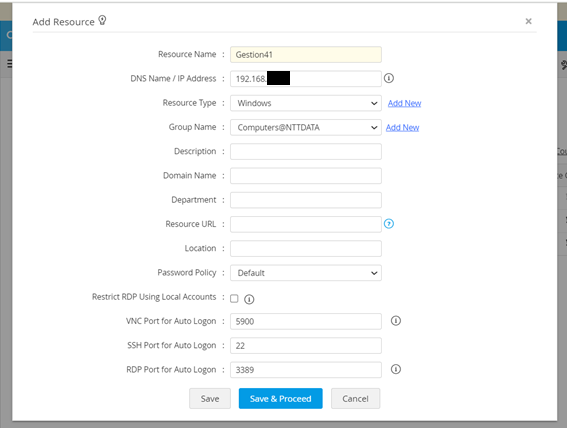
\includegraphics[width=0.8\textwidth]{./img/gestion41_importar.png}
	\caption{Gestión de contraseñas en PAM360.}
	\label{fig:gestion41_importar}
\end{figure}

\section{Gestión de contraseñas y acceso}
PAM360 se utilizó para gestionar contraseñas y controlar el acceso a diferentes recursos. La herramienta permitió la configuración de políticas de contraseñas y la asignación de roles a los usuarios. Esto aseguró que solo los usuarios autorizados pudieran acceder a ciertos recursos.

\begin{figure}[H]
	\centering
	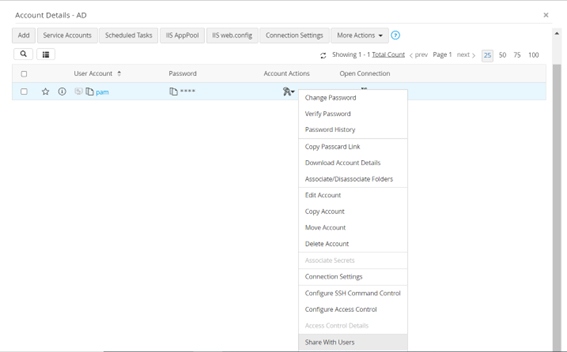
\includegraphics[width=0.8\textwidth]{./img/share_account_pam.png}
	\caption{Gestión de contraseñas en PAM360.}
	\label{fig:share_account_pam}
\end{figure}

Para conceder accesos en PAM es sencillo, se elige la cuenta de la máquina, la cual se va a ceder a un usuario. Seleccionamos la opción de "Share with Users".
Después, seleccionamos al usuario que le queremos dar acceso (en este caso, mi usuario)

\begin{figure}[H]
	\centering
	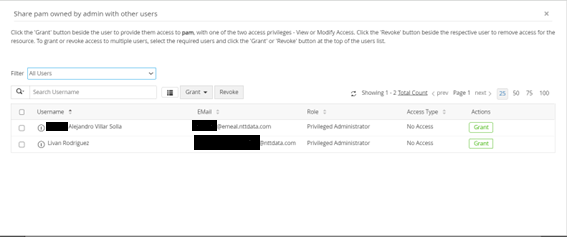
\includegraphics[width=0.8\textwidth]{./img/share_account_seleccion.png}
	\caption{Selección de usuario.}
	\label{fig:share_account}
\end{figure}

y seleccionamos la opción que deseemos, que sólo se pueda conectar a la máquina, que se pueda conectar y ver contraseñas o que pueda hacer todo incluso modificar contraseñas. Esta opciones varían dependiendo del tipo de privilegios que se le hayan concedido al usuario en PAM.

\begin{figure}[H]
	\centering
	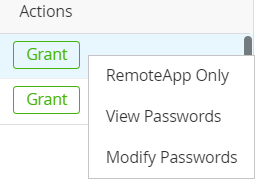
\includegraphics[width=0.8\textwidth]{./img/share-detail.png}
	\caption{Selección de usuario.}
	\label{fig:share_detail}
\end{figure}


Cuando tengamos contraseñas de máquinas guardadas y contraseñas asignadas, la portada de PAM cambiará y nos mostrará la información de nuestros sistemas

\begin{figure}[H]
	\centering
	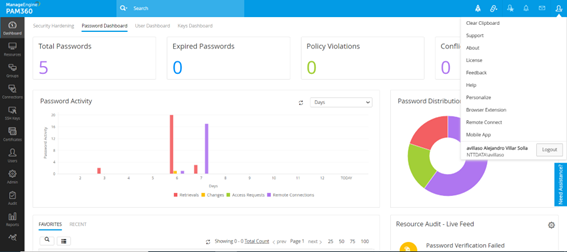
\includegraphics[width=0.8\textwidth]{./img/pam_portada_contodo.png}
	\caption{Configuración del administrador en PAM360.}
	\label{fig:pam_portadaactualizada}
\end{figure}

\section{Monitorización y auditoría}
Una vez configurado, PAM360 proporcionó capacidades de monitorización y auditoría que permitieron registrar todas las actividades de los usuarios. Esta funcionalidad es esencial para mantener la seguridad y cumplir con las políticas de la empresa.

El usuario accedería a la máquina a la cual tiene permiso. Introduciendo su usuario personal, tendría acceso a la máquina (en este caso Gestion42) como pam-access (cuenta la cual se ha creado para el uso de las máquinas). 

\begin{figure}[H]
	\centering
	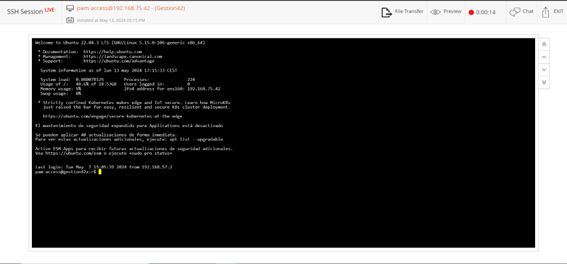
\includegraphics[width=0.8\textwidth]{./img/pam-ssh_live.png}
	\caption{Monitorización de actividades en PAM360.}
	\label{fig:pam_live}
\end{figure}

\begin{figure}[H]
	\centering
	\includegraphics[width=0.8\textwidth]{./img/pam_live.png}
	\caption{PAM360 configurado y operando.}
	\label{fig:pam_live2}
\end{figure}



\section{Resultados y validación}
Finalmente, se validó el correcto funcionamiento de PAM360 mediante pruebas exhaustivas. Dichas pruebas consistieron en mi tutor de la empresa y yo, cambiándonos los roles uno a otro, haciendo modificaciones en la máquina y el otro reportando dichas modificaciones para ver si se habían grabado correctamente. También se sometió a pruebas de penetración con Nessus y búsqueda de CVEs para PAM360, para comprobar si existía alguna vulnerabilidad. Se verificó que todos los usuarios importados pudieran acceder a los recursos según las políticas establecidas y que todas las actividades fueran registradas adecuadamente.Las acciones del usuario se quedan guardadas. Al acabar la sesión de uso pam proporciona reportes en modo de: PDF, html y vídeo.

También, el admin puede ver en tiempo real los movimientos que realizan los usuarios en las máquinas dentro de la propia solución.
\begin{figure}[H]
	\centering
	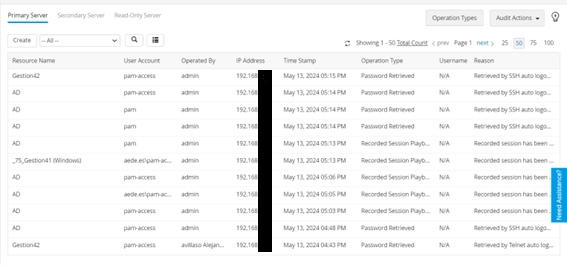
\includegraphics[width=0.8\textwidth]{./img/ad_movimientos.png}
	\caption{Monitorización de actividades en PAM360 en formato HTML.}
	\label{fig:ad_movimientos}
\end{figure}

Pero la información detallada sale al acabar la sesión
\begin{figure}[H]
	\centering
	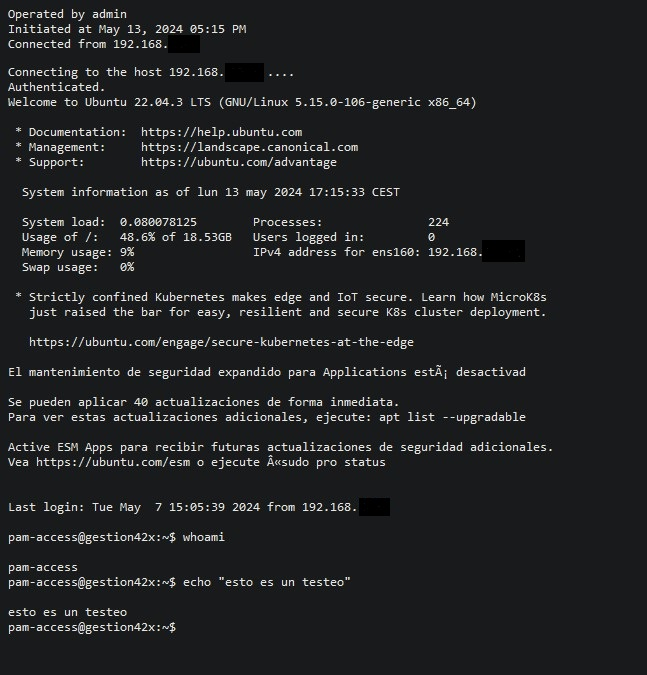
\includegraphics[width=0.8\textwidth]{./img/reporte_html.jpg}
	\caption{Resultados de la validación del sistema.}
	\label{fig:reporte_html}
\end{figure}



